\documentclass{article}

\usepackage{url}

\usepackage{times}
\usepackage{amsthm}
\usepackage{amsmath}
\usepackage{amssymb}

\usepackage[font=footnotesize]{caption}
\usepackage[font=footnotesize]{subcaption}
\usepackage[pdftex]{graphicx}
\usepackage{wrapfig}
\usepackage{epstopdf}
\usepackage[american]{babel}
\usepackage{url}
\usepackage{color}
\usepackage{xspace}
\usepackage{float}
\usepackage{tabularx}
\usepackage{multirow}
\usepackage{alltt}
\usepackage{multicol}
\usepackage{blindtext}
\usepackage{scrextend}
\usepackage{geometry}
\addtokomafont{labelinglabel}{\sffamily}

\usepackage{algorithmic}
\renewcommand{\algorithmiccomment}[1]{// #1} % Brackets are confused with the sets
\usepackage{algorithm} % For counting chapters
\algsetup{linenosize=\scriptsize}
\xspaceaddexceptions{=}
\xspaceaddexceptions{\}}
\xspaceaddexceptions{\in}

\geometry{margin=1in}

% A set depicted with bold:
\newcommand{\set}[1]{\ensuremath{\mathbf{#1}}\xspace}

% The elements of a set:
\newcommand{\elements}[3]{\ensuremath{\{#1_{#2},...,#1_{#3}\}}\xspace} 

%The cardinality of a given set belonging somewhere:
\newcommand{\cardinality}[2]{\ensuremath{|\set{#1}_{#2}|}\xspace} 		

% A mathematical unit:
\newcommand{\unit}[1]{\ensuremath{\mathrm{#1}}\xspace} 	

\DeclareMathOperator*{\argmin}{arg\,min}

\newtheorem{definition}{Definition}

% correct bad hyphenation here
\hyphenation{}

\title{An empirical investigation of peremptory challenge}
\author{Christopher Salahub}

\begin{document}
\maketitle

\section{Introduction} \label{sec:Intro}

The Gerald Stanley murder trial was noteworthy for all of the wrong reasons. The first reason was the crime itself. The rural
region around Biggar, Saskatchewan\cite{StanleyWitnessAccounts} is not known for crime, indeed, the crime statistics collected by
Statistics Canada suggest it is one of the safest in the province\cite{SaskatchewanCrime}. Any murder at all would be worthy of
attention and subject to plenty of drama. But beyond the damage this trial has done to the community, this trial is noteworthy
because it led to a significant re-examination of the legal jurisprudence surrounding the jury selection process culminating in
the proposition of Bill C-75 by the Canadian government in March of 2018\cite{billc75}, less than two months after the trial's
verdict\cite{GeraldStanleyVerdict}.

Bill C-75, in part, aims to ameliorate one of the critical points of contention about the Gerald Stanley case: the use of
peremptory challenges in jury selection. The outsized impact of the case was due, in large part, to it's racial aspect. Gerald
Stanley, a white man, was accused of second degree murder in the killing of Colten Boushie, a First Nations man. Given Canada's
troubled history with First Nations groups, this alone would have been enough to make the trial a flash point for race issues, but
that was not the worst aspect of the trial. Rather, it was the alleged use of peremptory challenges to strike five potential
jurors who ``appeared'' to be First Nations, resulting in an all-white jury, that proved to be the most controversial and
influential facet of the entire affair\cite{fiverejected} \cite{fraughthistory}.

With Bill C-75 currently moving through the Canadian parliamentary system, having completed its second reading in June
2018\cite{c75legisinfo}, a close re-examination of the practice of peremptory challenge is warranted. A great deal of ink has
already been spilled on both sides of the debate \cite{peremparegood} \cite{bothwrong} \cite{goodfirststep}, but startlingly
little of this discussion has been based on any hard evidence on the impact of peremptory challenge in jury selection. This paper
aims to provide analysis and evidence to illuminate the topic further by analyzing three separate peremptory challenge
data sets collected in the United States \cite{JurySunshineProj} \cite{StubbornLegacy} \cite{PerempChalMurder}. While this data
cannot tell us if challenges were racially motivated in the Stanley trial, stepping back from this fraught legal episode to take a
wider view of the practice of peremptory challenge provides a more sober place to start the discussion of its place in modern jury
trials.

This paper will proceed in five parts. Section \ref{sec:background} provides a brief history of the practice of peremptory
challenges in jury trials, in particular explaining their original motivation and past implementations in \ref{subsec:history} and
how they have developed in the United States, the United Kingdom, and Canada in \ref{subsec:modprac}. Section \ref{sec:data}
proceeds to discuss the three data sets obtained, with \ref{subsec:jspdata} -- \ref{subsec:phillydata} discussing the sources and
collection methods before the cleaning and preprocessing are explained in \ref{subsec:datacleaning}. Section \ref{sec:analysis}
then provides the details and results of the different analyses performed on the different data sets, before these results are
compared to previous works in Section \ref{sec:comparison}. Finally, the results and findings are summarized in
\ref{sec:conclusion}, and recommendations based on the observations obtained here are provided.

\section{Background} \label{sec:background}

\subsection{History of Peremptory Challenge} \label{subsec:history}

\subsection{Modern Practice} \label{subsec:modprac}

\section{Data} \label{sec:data}

\subsection{Jury Sunshine Project} \label{subsec:jspdata}

\subsection{North Carolina Data} \label{subsec:norcardata}

\subsection{Philadelphia Data} \label{subsec:phillydata}

\subsection{Data Cleaning} \label{subsec:datacleaning}

\textbf{Jury Sunshine Data}

The data collected in North Carolina proved invaluable to this project \cite{JurySunshineProj}.

\underline{Problem}: some columns of the data contained only NA values
\underline{Solution}: \texttt{lapply} to remove these uninformative columns

\underline{Problem}: relational database provided did not have all data in one joined table
\underline{Solution}: creation of \texttt{CleaningMerge} function: a wrapper for \texttt{merge} which provides information about the
mismatches which may be present in the two merged tables

\underline{Problem}: inconsistently coded levels, e.g. inconsistent case or ``?'' instead of ``U'' for unknowns
\underline{Solution}: forcing levels to be uppercase and the replacement of obvious mis-specified levels

\underline{Problem}: some columns seem to have swapped values, e.g. the gender column should be one of ``M'', ``F'', or ``U'' and the
political affiliation column should be one of ``D'', ``R'', ``I'', or ``U'', but some individuals have the gender recorded as
``R'' and political affiliation as ``M''
\underline{Solution}: the creation of the \texttt{IdentifySwap} function, which has two arguments: a data set and the acceptable or correct
levels for the variables in the data set. It then identifies rows which have candidate swaps and presents them for review

\section{Analysis} \label{sec:analysis}

\subsection{Modelling} \label{subse:mods}

In order to create a single model to test the statistical significance of the differences observed for strike rates by race,
defendant race, and party doing the striking, a saturated poisson regression model was fit to the data. Letting $i$ denote the
level of the venire member race, $j$ the defendant race, and $k$ the disposition, the numbers of observed venire members in each
$ijk$ combination, $y_{ijk}$ were modelled as Poisson-distributed random variables with expectation $\lambda_{ijk}$. A saturated
model was then fit to the data, that is a model described by the equation:

$$\log{E[y_{ijk}]} = \textbf{x}_{ijk}\beta = \beta_o + \beta_R x_{i..} + \beta_{D} x_{.j.} + \beta_S x_{..k} + \beta_{R:D}
x_{i..} x_{.j.} + \beta_{R:S} x_{i..} x_{..k} +\beta_{D:S} x_{.j.} x_{..k} + \beta_{R:D:S} x_{i..} x_{.j.} x_{..k}$$

Where $x_{i..}$ indicates the race level of the $ijk$ cell, and $x_{.j.},x_{..k}$ are defined analogously for the defendant race
and disposition. The interaction terms then serve to answer questions about the racial pattern of strikes which is utilized by
each party given the defendant race. Most interesting to this investigation is the third order interaction term. This term
indicates a significant difference in racial strike patterns given the party striking and the defendant race. In other words, this
term accounts for different patterns for the different parties which are not independant of the defendant race.

When this term is tested using a nested model without the third order interaction, the third order interaction is found to be
significant. This suggests that not only do the patterns present in the different parties vary, but they vary differently for
different defendant races. This dependence can be viewed using a novel graphic presented in Figure \ref{fig:raceraceparcoord}.

\begin{figure}[!h]
  \centering
  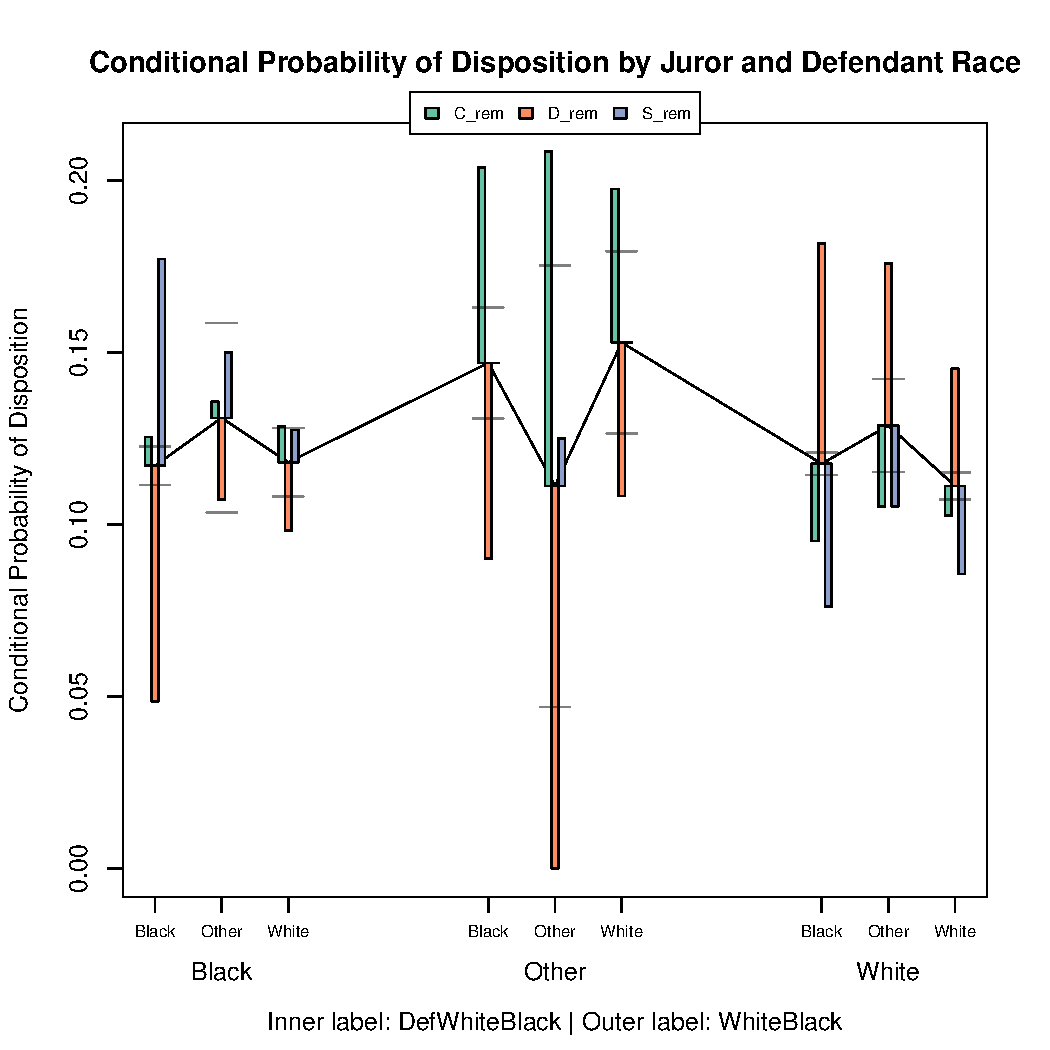
\includegraphics[width=0.7\linewidth]{Plots/CondDistRaces}
  \caption{Parallel coordinate plot of racial strike tendencies}
  \label{fig:raceraceparcoord}
\end{figure}

The conditional probability of a particular disposition given the racial combination of venire person and defendant is displayed
on the y-axis, that is the count of individuals for a particular race, defendant race, and disposition combination divided by the
number of individuals with the racial combination across all dispositions. The x-axis then displays the combinations, grouped by
the venire member race to show the dominant pattern in the data.

The black line running across the plot is the mean, or expected, rejection probability that all parties would have if they acted
identically. That is, the relative level of this line provides the relative strike rate on aggregate for a particular racial
combination. The bars extending from this line at each point go from this line to the corresponding value of the party represented
by the bar. Finally, the horizontal lines provide approximate confidence intervals for each combination\footnote{Generated
  assuming a binomial distribution of struck (by any party) against kept, as when this data is modelled with a poisson
  distribution, the distribution of sub-processes given the overall count will be binomially distributed}.

The dominant pattern to these strikes is a tendency of the defense to preferentially reject white venire members and keep black
venire members, and of the prosecution to do the opposite. It was already noted in the literature\cite{JurySunshineProj}, but the
addition of defendant race allows us to make a stronger statement, as this pattern remains across defendant races. It also adds
nuance, however, as the race of the defendant has a clear impact on the lengths of the bars for both the defense and
prosecution. The prosecution seems to favour a jury which does not match the race of the defendant, while the defense seems to
favour a jury which does.

While this second tendency seems to have no justification beyond race, the dominant tendency may have other justification than
simply skin colour. As was noted by ``Ideological Imbalance and Peremptory Challenge'', black individuals are more consistently
aligned with the democratic party, and as a consequence a lawyer which suspects this political bias will impact the trial outcome
would preferentially strike or keep black jurors in order to keep as many left wing individuals as possible. In this data, this
political imbalance is incredibly prevalent, as can be seen in Figure \ref{fig:racepolitics} \textcolor{red}{Add the plot of this
  effect here, elaborate on this pattern more based on the plot}.

\begin{figure}[!h]
  \centering
  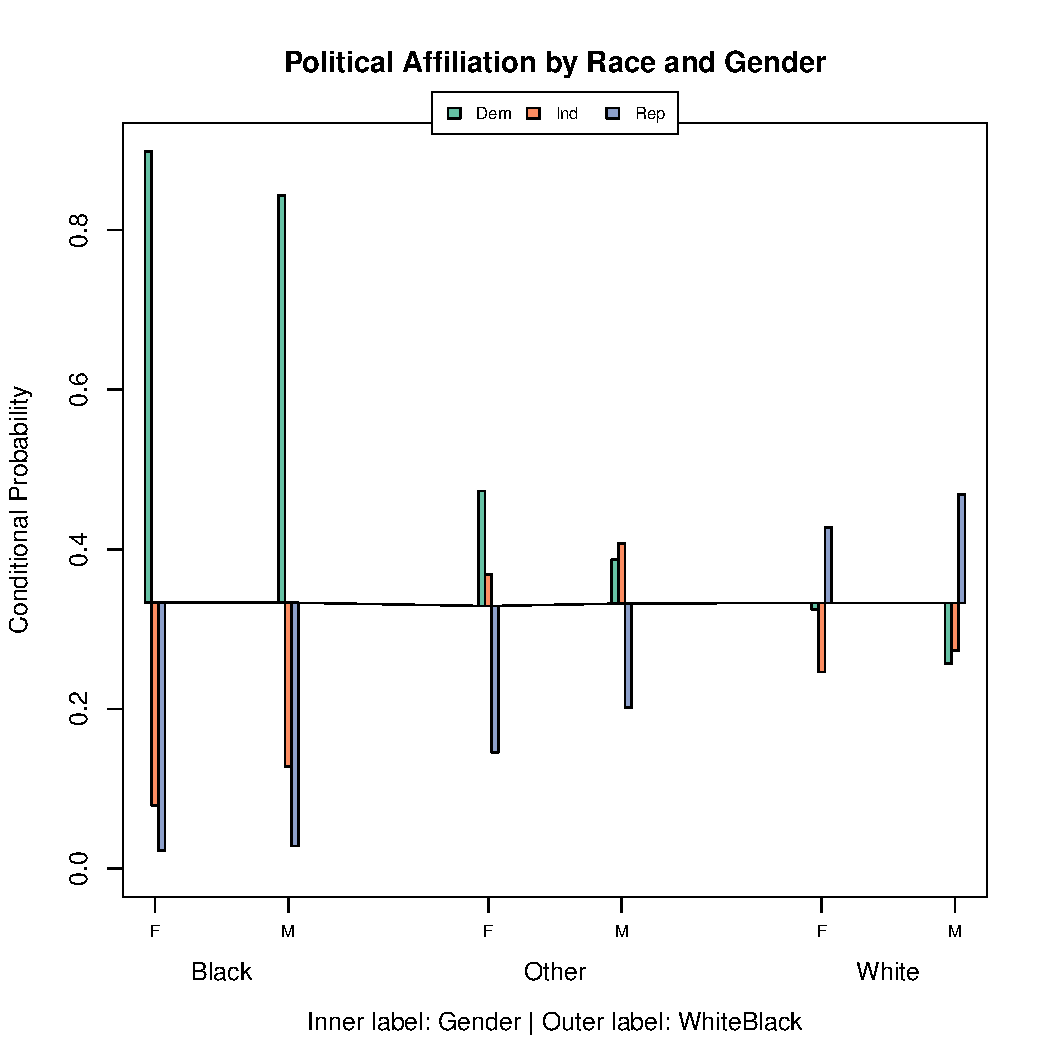
\includegraphics[width=0.7\textwidth]{Plots/RaceGenderPolit}
  \caption{Conditional probabilities of political affiliation by race and gender}
  \label{fig:racepolitics}
\end{figure}

Perhaps more interestingly, the prosecution and judge seem to match in their tendency from the mean at every combination. This
suggests that both challenges with cause and the prosecution tend to have the same effect on the jury composition, though the
magnitudes can differ greatly for these two strikes.

\section{Comparison to Previous Work} \label{sec:comparison}

\section{Conclusions and Recommendations} \label{sec:conclusion}

\section{Ideas}
\begin{itemize}
\item look at the CSI from StatsCan, or an analogous US value, to assess the severity of a crime
\item Kullback-Leibler divergence of accepted jury distribution to the venire distribution
\item Look at guilty verdict tendencies based on jury race vs. defendant race
\end{itemize}

\bibliographystyle{abbrv}
\bibliography{perempchallenge} 

\end{document}